\section{The robotic setup}
\label{Sec:setup}

\begin{figure}
\centering
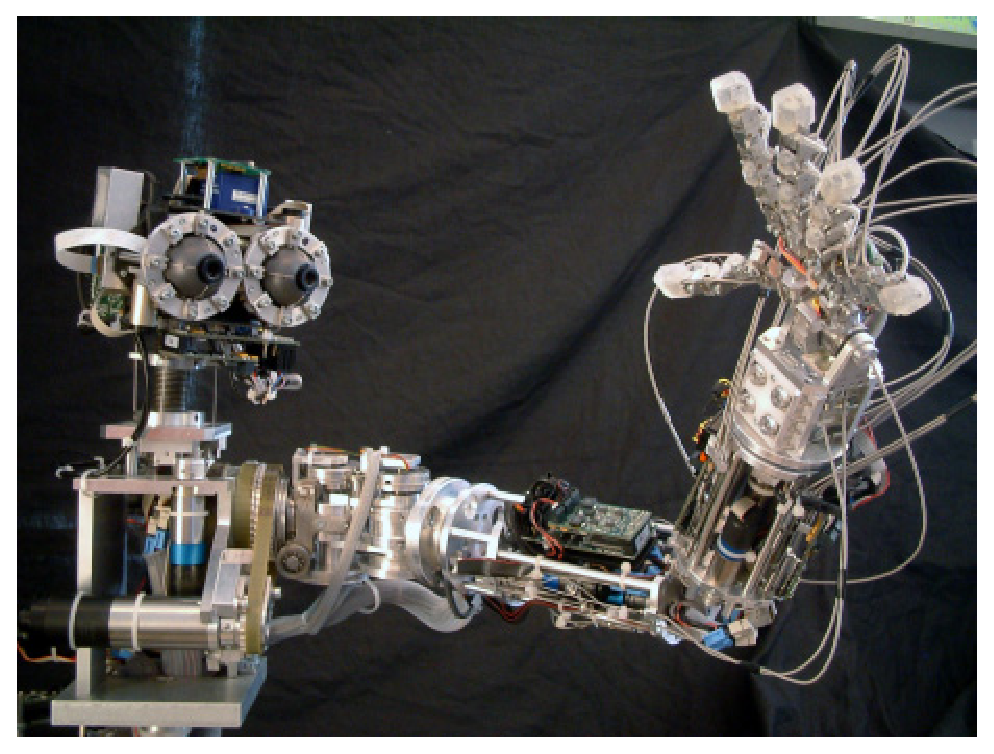
\includegraphics[width=60mm]{Figure/James1.eps}
\caption{The humanoid robot James.}
\label{Fig:PicureJames}
\end{figure}

The experiments described in this paper were carried out on the robot 
James (see figure \ref{Fig:PicureJames}). James is an upper body 
humanoid robot which consists of 22 DOFs, actuated by a total of 
23 motors. Torque is transmitted to the joints by belts and 
stainless-steel tendons. The head is equipped with two eyes, which 
can pan and tilt independently (4 DOFs), and is mounted on a 3-DOF 
neck. The arm has 7 DOFs: three of them are located in the shoulder, 
one in the elbow and three in the wrist. The hand has five fingers 
and is under-actuated with a total of 20 degrees of freedom controlled 
by 8 motors. 

The head structure has a total of 7 degrees of freedom, actuated by 8 
motors. Four of these motors are used to independently actuate the pan 
and tilt movements of the left and right eyes. Even though the eyes 
can be moved independently, our strategy was to couple their movements 
so to achieve a more human-like motion. We used common tilt 
$\alpha_t^c$, vergence $\alpha_v^d$ and version $\alpha_v^c$. 

The neck has three degrees of freedom, denoted $\theta_y$, 
$\theta_p$ and $\theta_r$ for yaw, pitch and roll respectively. These 
two rotations are achieved with an unconventional actuation structure 
(see for a detailed description \cite{jamone06james}). 

To summarize, the variables relevant to understand the remainder of the paper
are: the head joints 
$\mathbf q_{head}$ = $\begin{bmatrix} \alpha_t^c & \alpha_v^d & \alpha_v^c & \theta_y & \theta_p & \theta_r \end{bmatrix}^\top \in \mathbb R^6$ and the first four arm joints (3 d.o.f. shoulder and elbow) denoted $\mathbf q_{arm} \in \mathbb R^4$.
